\documentclass{article}[12pt]

% useful packages
\usepackage{fullpage}
\usepackage{amsmath,amssymb,amsthm,amsfonts}
\usepackage{graphicx}
\usepackage{enumerate}
\usepackage{algorithm,algorithmic}
\usepackage{xcolor}
\usepackage{bbm}
\usepackage{url}
\usepackage{caption,subcaption}

% theorem type environments
\newtheorem{thm}{Theorem}
\newtheorem{prop}{Proposition}
\newtheorem{lemma}{Lemma}
\newtheorem{cor}{Corollary}
\newtheorem{defn}{Definition}
\newtheorem{assump}{Assumption}
\newtheorem{example}{Example}
\newtheorem{conjecture}{Conjecture}

% frequently used symbols
\newcommand{\bE}{\mathbb{E}}
\newcommand{\bP}{\mathbb{P}}
\newcommand{\bQ}{\mathbb{Q}}
\newcommand{\bR}{\mathbb{R}}
\newcommand{\bS}{\mathbb{S}}
\newcommand{\bN}{\mathbb{N}}
\newcommand{\bZ}{\mathbb{Z}}
\newcommand{\sC}{{\mathcal C}} 
\newcommand{\sD}{{\mathcal D}} 
\newcommand{\sE}{{\mathcal E}} 
\newcommand{\sF}{{\mathcal F}} 
\newcommand{\sL}{{\mathcal L}} 
\newcommand{\sH}{{\mathcal H}} 
\newcommand{\sN}{{\mathcal N}} 
\newcommand{\sO}{{\mathcal O}} 
\newcommand{\sP}{{\mathcal P}} 
\newcommand{\sR}{{\mathcal R}} 
\newcommand{\sS}{{\mathcal S}}
\newcommand{\sU}{{\mathcal U}} 
\newcommand{\sX}{{\mathcal X}} 
\newcommand{\sY}{{\mathcal Y}} 
\newcommand{\sZ}{{\mathcal Z}}

% operators
\newcommand{\sign}{\mathop{\mathrm{sign}}}
\newcommand{\supp}{\mathop{\mathrm{supp}}} % support
\newcommand{\argmin}{\operatornamewithlimits{arg\ min}}
\newcommand{\argmax}{\operatornamewithlimits{arg\ max}}
\newcommand{\dist}{\operatorname{dist}}
\newcommand{\tr}{\text{tr}}
\newcommand{\vecop}{\text{vec}}
\newcommand{\st}{\operatorname{s.t.}}
\newcommand{\cut}{\setminus}
\newcommand{\ra}{\rightarrow}
\newcommand{\ind}[1]{\mathbbm{1}\left\{#1\right\}} 
\newcommand{\given}{\ | \ }

% grouping operators
\newcommand{\brac}[1]{\left[#1\right]}
\newcommand{\set}[1]{\left\{#1\right\}}
\newcommand{\abs}[1]{\left\lvert #1 \right\rvert}
\newcommand{\paren}[1]{\left(#1\right)}
\newcommand{\norm}[1]{\left\|#1\right\|}
\newcommand{\ip}[2]{\left\langle #1,#2 \right\rangle}

% code commands
\newcommand{\matlab}{\textsc{Matlab }}
\newcommand{\algname}[1]{\textnormal{\textsc{#1}}}

% header command
\newcommand{\homework}[4]{
    \pagestyle{myheadings}
    \thispagestyle{plain}
    \newpage
    \setcounter{page}{1}
    \setlength{\headsep}{10mm}
    \noindent
    \begin{center}
    \framebox{
        \vbox{\vspace{2mm}
            \hbox to 6.28in { {\bf STAT 672: Statistical Learning I
            \hfill Winter 2020} }
        \vspace{4mm}
        \hbox to 6.28in { {\Large \hfill Homework #1 \hfill} }
        \vspace{2mm}
        \hbox to 6.28in { \Large \hfill Due: #2 \hfill }
        \vspace{2mm}
        \hbox to 6.28in { {\it Student Name: #3} \hfill {\it Professor Name: #4}}
        \vspace{2mm}}
   }
   \end{center}
   \markboth{Homework #1}{Homework #1}
   \vspace*{4mm}
}

\begin{document}

\homework{1}{January 29th, 2020}{Ethan Lew}{Bruno Jedynak}

\section{Orthogonal Projection in a Hilbert Space}
Let $H$ be a Hilbert space and $V$ a closed subspace of $H$. Notate $\pi_V(f)$ the orthogonal projection of $f$ onto $H$. $\pi_V(f)$ is then the unique element of $H$ which verifies:
\begin{enumerate}
\item $\pi_V(f) \in V$;
\item $\langle f-\pi_V(f),g\rangle=0$ for all $g \in V$;
\end{enumerate}
Show the following: 
\begin{enumerate}
\item for any $f \in H$, $||f||^2 = ||\pi_V(f)||^2 + ||f-\pi_V(f)||^2$

\textbf{Solution:} First, recall that
\begin{equation}
	||f||_{\mathcal H}^2 = \langle f, f \rangle_{\mathcal H}.
\end{equation}
Now, manipulate the RHS of the equation,
\begin{equation}
	\begin{aligned}
		||\pi_V(f)||^2 + ||f-\pi_V(f)||^2 &= ||\pi_V(f)||^2 + \langle f, f \rangle - 2 \langle f, \pi_V(f) \rangle + \langle \pi_V(f), \pi_V(f) \rangle \\
		  &= || f ||^2 + 2 \left( \langle f, \pi_V(f) \rangle - \langle \pi_V(f), \pi_V(f) \rangle \right) \\
		  &= ||f||^2 + 2  \langle f - \pi_V(f), \pi_V(f) \rangle \\
	\end{aligned} 
\end{equation}
As $\pi_V(f) \in V$,
\begin{equation}
	||\pi_V(f)||^2 + ||f-\pi_V(f)||^2 = ||f||^2.
\end{equation}

	
\item for any $f,g \in H$, $\langle f,\pi_V(g)\rangle=\langle g,\pi_V(f)\rangle$

Hint: verify that $\langle f,\pi_V(g)\rangle=\langle\pi_V(f),\pi_V(g)\rangle$, similarly for the right hand side and conclude.

\textbf{Solution:} From the second condition, it is evident that
\begin{equation}
	\begin{aligned}
		\langle f - \pi_V(f), g \rangle &= \langle g - \pi_V(g), f \rangle \\
		\langle f, g \rangle - \langle g, \pi_V(f) \rangle &= \langle g, f \rangle - \langle f, \pi_V(g) \rangle \\
\langle g, \pi_V(f) \rangle &= \langle f, \pi_V(g) \rangle \\
	\end{aligned}
\end{equation}

\item provide an example of a Hilbert space $H$ and a subspace $V$ which is not closed in $H$ and provide $f \in H$ such that $\pi_V(f)$ does not exist. 
\end{enumerate}

\section{A Reproducing Kernel is Positive Definite}
Let $H$ be a RKHS of functions $\mathcal{X} \mapsto \mathbb{R}$ with reproducing kernel K. This means that 
\begin{enumerate}
\item for any $y \in \mathcal{X}$, $K(.,y) \in H$
\item for any $f \in H$, and $y \in \mathcal{X}$, $\langle f, K(.,y) \rangle = f(y)$
\end{enumerate}

Show the following: 
\begin{enumerate}
\item $K$ is symmetric;
Hint: verify that for any $x,y \in \mathcal{X}$, $\langle K(.,x), K(.,y) \rangle = K(x,y)$

\textbf{Solution:} The reproducing property holds that, 
\begin{equation}
	\langle f, K(., y) \rangle = f(y)
\end{equation}
Apply the reproducing property to the LHS of the hint,
\begin{equation}
	\begin{aligned}
		\langle K(.,x), K(., y) \rangle = K(x, y).
	\end{aligned}
\end{equation}
So, then, symmetry can be found trivially,
\begin{equation}
	\begin{aligned}
		K(x, y) &= \langle K(., x), K(., y) \rangle \\
			&= \langle K(., y), K(., x) \rangle \\
			&= K(y, x).
	\end{aligned}
\end{equation}

\item $K$ is positive definite; 

\textbf{Solution:} A kernel, $K$, is said to be positive definite if, for any $\alpha_1, ..., \alpha_m \in \mathbb R, x_1, ..., x_m \in \mathcal X$ the following condition holds,
\begin{equation}
	\sum^{m}_{i=1} \sum^{m}_{j=1} \alpha_i \alpha_j K(x_i, x_j) \ge 0. 
\end{equation}
The LHS can be manipulated as 
\begin{equation}
	\begin{aligned}
		\sum^{m}_{i=1} \sum^{m}_{j=1} \alpha_i \alpha_j K(x, y)  &= \sum^{m}_{i=1} \sum^{m}_{j=1} \alpha_i \alpha_j \langle K(., x_i), K(., x_j) \rangle \\    
									 &=  \langle \sum^{m}_{i=1} \alpha_i K(., x_i), \sum^{n}_{i=1}, \sum^{m}_{j=1} \alpha_j K(., x_j)    \rangle \\
									 &= \left| \left| \sum^{m}_{i=1} \alpha_i K(., x_i)  \right| \right|^2
	\end{aligned}
\end{equation}
This norm is always non-negative, so it can be concluded that
\begin{equation}
	\sum^{m}_{i=1} \sum^{m}_{j=1} \alpha_i \alpha_j K(x_i, x_j) \ge 0, 
\end{equation}
meaning that the kernel satisfies the positive definite property.



\item for any $f \in H$ and $x \in \mathcal{X}$, $|f(x)|\leq ||f||\sqrt{K(x,x)}$

Hint: use the reproducing property to write $f(x)$ as an inner product than use the Cauchy-Schwarz inequality. 
\end{enumerate}

\textbf{Solution:} The Cauchy-Schwarz inequality holds that for two elements, $v, f \in \mathcal H$, the following condition holds 
\begin{equation}
	\langle f, g \rangle_{\mathcal H} \le || f ||_{\mathcal H} || g ||_{\mathcal H}.
\end{equation}

Consequently, the reproducing property can yield an equality for $f(x)$ for which the Cauchy-Schwarz inequality can be applied,
\begin{equation}
	\begin{aligned}
		f(x) &= \langle f, K(., x) \rangle_{\mathcal H} \\
		     &\le || f||_{\mathcal H} ||K(., x)||_{\mathcal H}. \\
	\end{aligned}
\end{equation}
The factor $|| K(., x) ||_{\mathcal H}$ can be manipulated as
\begin{equation}
	\begin{aligned}
	|| K(., x) ||^2_{\mathcal H} &= \langle K(., x), K(., x) \rangle \\
				     &= K(x, x).
	\end{aligned}
\end{equation}
Accounting for the sign of the square root term,
\begin{equation}
	|f(x)| \le ||f||_{\mathcal H} \sqrt{K(x,x)}.
\end{equation}

\section{RKHS Over a Finite Set}
Let $\mathcal{X} = \{-m,\ldots,-1,0,1,\ldots,m\}$. Let $K$ be a positive definite kernel over $\mathcal{X}$ for which the $(2m+1,2m+1)$ matrix $K$ such that $K_{ij}=K(i,j)$ is invertible. We have seen in class that the RKHS with reproducing kernel $K$ is the vector space $\mathbb{R}^{2m+1}$ with inner product, 
$$\langle f,g \rangle = f^T K^{-1}g $$
where $f=(f_1,\ldots,f_{2m+1})^T$ and $f_i=f(i-m-1)$ and similarly for $g$. 
One can then sample elements of $H$ according to the following probability distribution:  
$$p(f) = C e^{-\frac{||f||_H^2}{2}}$$
where $C>0$ is a constant. 
\begin{enumerate}
\item This distribution is Multivariate Normal MVN$(\mu,\Sigma)$. What are the parameters $\mu$ and $\Sigma$?

\textbf{Solution:} MVN$(\mu, \Sigma)$ PDF can be defined as 
	\begin{equation}
		p(x) = \frac{1}{(2\pi)^{k/2} \text{det}(\Sigma)^{1/2}} e^{- \frac{1}{2} (x-\mu)^T \Sigma^{-1} (x-\mu) }. 
	\end{equation}
From the distribution of sample elements, it can be observed that 
	\begin{equation}
		\begin{cases}
			\mu &= \mathbf 0 \\	
			K &= \Sigma \\
		\end{cases}.
	\end{equation}

\item What is the constant $C$?

\textbf{Solution:} Comparing the MVN form against the sample distribution, it is evident that 
	\begin{equation}
		C = \frac{1}{(2\pi)^{m+1/2} \text{det} (K)^{1/2}}. 
	\end{equation}
	
\item Show some samples for the following kernels
\begin{enumerate}
\item Gaussian kernel $K_\tau(i,j)=e^{-\frac{1}{2\tau^2}(i-j)^2}$

\textbf{Solution:} See Figure \ref{fig:example}.

\item Show more examples with the same kernel and different parameter $\tau$. Comment on the results. 

\textbf{Solution:} See Figure \ref{fig:example}. For higher values of $\tau$, the function appears smoother. 

\item Show more examples with 2 different kernels of your choice. 

\textbf{Solution:} See Figure \ref{fig:example}. The polynomial kernel (for order 2) and min function were chosen.

\begin{figure}%
    \centering
    \subfloat[Gaussian Kernel with Two $\tau$ Values]{{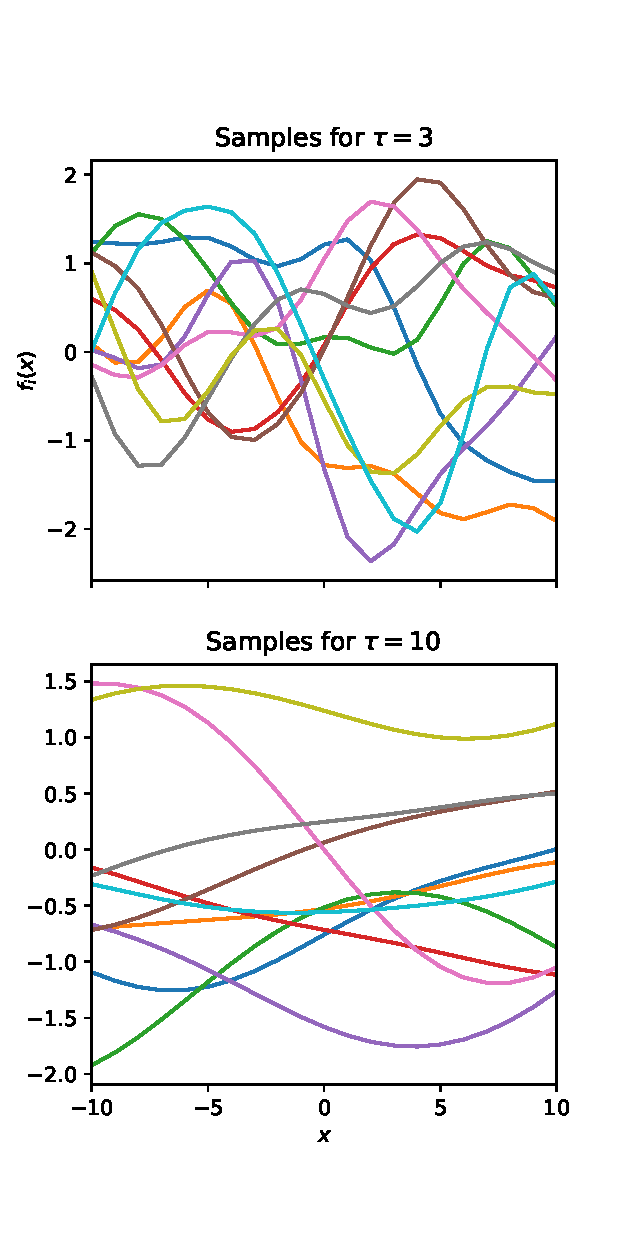
\includegraphics[width=7cm]{./img/gaussian_kernel_fig.eps} }}%
    \qquad
    \subfloat[Other Kernels]{{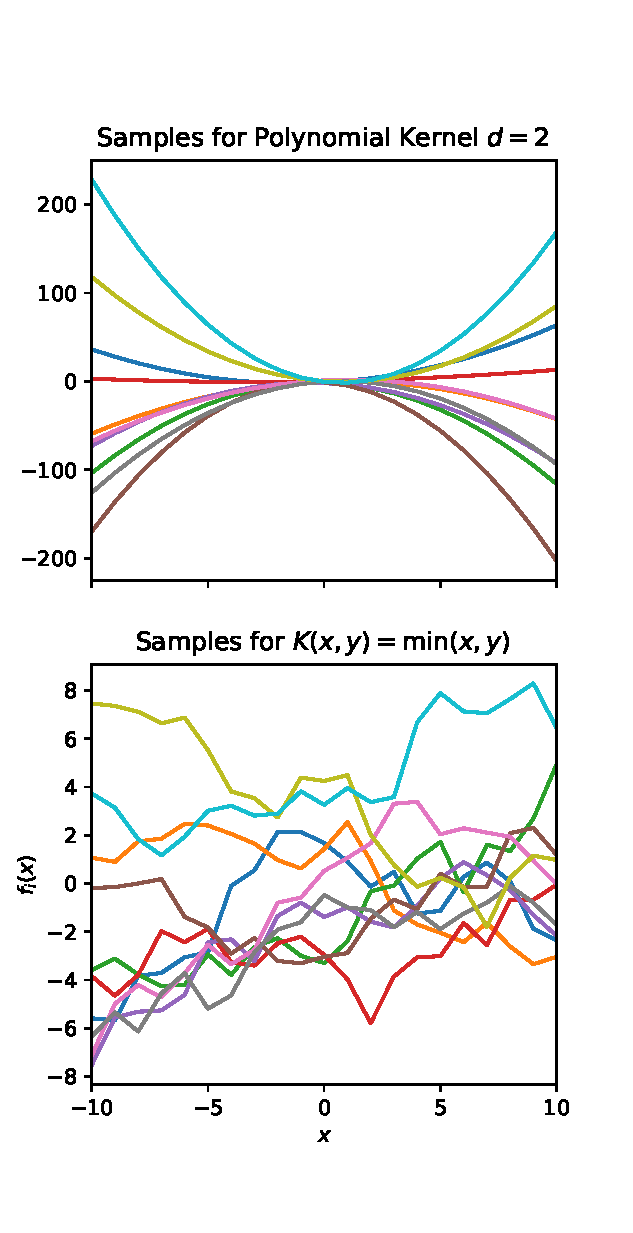
\includegraphics[width=7cm]{./img/other_kernel_fig.eps} }}%
    \caption{Problem 3 Plots of Random Process Samples}%
    \label{fig:example}%
\end{figure}

%\begin{figure}
%	\centering 
%\includegraphics[width=0.7\textwidth]{./Gauss.pdf}
%\caption{\label{fig:Gauss}Example of 10 samples of functions of the RKHS over $\{-10,\ldots,10\}$ with the Gaussian kernel, $\tau=10$.}
%\end{figure}
\end{enumerate}
\end{enumerate} 
\end{document}
